\documentclass[pdf,distiller]{prosper}
\usepackage[toc,highlight,HA]{HA-prosper}

% For eps figure replacements
\usepackage{psfrag}
% For AMS symbols and equations
\usepackage{amssymb,amsmath}

% Load the graphicx package
\usepackage{graphicx}

%%% Example macros (some are not used in this sample file) %%%

% For units of measure
\newcommand\dynpercm{\nobreak\mbox{$\;$dynes\,cm$^{-1}$}}
\newcommand\cmpermin{\nobreak\mbox{$\;$cm\,min$^{-1}$}}
\newcommand\mpers{\nobreak\mbox{$\;$m\,s$^{-1}$}}
\newcommand\meters{\nobreak\mbox{$\;$m}}
\newcommand\persec{\nobreak\mbox{$\;$s$^{-1}$}}
\newcommand\mperss{\nobreak\mbox{$\;$m\,s$^{-2}$}}

% Various bold symbols
\providecommand\bnabla{\boldsymbol{\nabla}}
\providecommand\bcdot{\boldsymbol{\cdot}}
\newcommand\biS{\boldsymbol{S}}
\newcommand\etb{\boldsymbol{\eta}}

% For multiletter symbols
\newcommand\Real{\mbox{Re}} % cf plain TeX's \Re and Reynolds number
\newcommand\Imag{\mbox{Im}} % cf plain TeX's \Im
\newcommand\Rey{\mbox{\textit{Re}}}  % Reynolds number
\newcommand\Pran{\mbox{\textit{Pr}}} % Prandtl number, cf TeX's \Pr product
\newcommand\Pen{\mbox{\textit{Pe}}}  % Peclet number
\newcommand\Ai{\mbox{Ai}}            % Airy function
\newcommand\Bi{\mbox{Bi}}            % Airy function

% For sans serif characters:
% The following macros are setup in JFM.cls for sans-serif fonts in text
% and math.  If you use these macros in your article, the required fonts
% will be substitued when you article is typeset by the typesetter.
%
% \textsfi, \mathsfi   : sans-serif slanted
% \textsfb, \mathsfb   : sans-serif bold
% \textsfbi, \mathsfbi : sans-serif bold slanted (doesnt exist in CM fonts)
%
% For san-serif roman use \textsf and \mathsf as normal.
%
\newcommand\ssC{\mathsf{C}}    % for sans serif C
\newcommand\sfsP{\mathsfi{P}}  % for sans serif sloping P
\newcommand\slsQ{\mathsfbi{Q}} % for sans serif bold-sloping Q

% Hat position
\newcommand\hatp{\skew3\hat{p}}      % p with hat
\newcommand\hatR{\skew3\hat{R}}      % R with hat
\newcommand\hatRR{\skew3\hat{\hatR}} % R with 2 hats
\newcommand\doubletildesigma{\skew2\tilde{\skew2\tilde{\Sigma}}}
%       italic Sigma with double tilde

% array strut to make delimiters come out right size both ends
\newsavebox{\astrutbox}
\sbox{\astrutbox}{\rule[-5pt]{0pt}{20pt}}
\newcommand{\astrut}{\usebox{\astrutbox}}

\newcommand\GaPQ{\ensuremath{G_a(P,Q)}}
\newcommand\GsPQ{\ensuremath{G_s(P,Q)}}
\newcommand\p{\ensuremath{\partial}}
\newcommand\tti{\ensuremath{\rightarrow\infty}}
\newcommand\kgd{\ensuremath{k\gamma d}}
\newcommand\shalf{\ensuremath{{\scriptstyle\frac{1}{2}}}}
\newcommand\sh{\ensuremath{^{\shalf}}}
\newcommand\smh{\ensuremath{^{-\shalf}}}
\newcommand\squart{\ensuremath{{\textstyle\frac{1}{4}}}}
\newcommand\thalf{\ensuremath{{\textstyle\frac{1}{2}}}}
\newcommand\Gat{\ensuremath{\widetilde{G_a}}}
\newcommand\ttz{\ensuremath{\rightarrow 0}}
\newcommand\ndq{\ensuremath{\frac{\mbox{$\partial$}}{\mbox{$\partial$} n_q}}}
\newcommand\sumjm{\ensuremath{\sum_{j=1}^{M}}}
\newcommand\pvi{\ensuremath{\int_0^{\infty}%
  \mskip \ifCUPmtlplainloaded -30mu\else -33mu\fi -\quad}}

\newcommand\etal{\mbox{\textit{et al.}}}
\newcommand\etc{etc.\ }
\newcommand\eg{e.g.\ }


\newtheorem{lemma}{Lemma}
\newtheorem{corollary}{Corollary}

\newcommand{\bol}[1]{\ensuremath{\mathbf{#1}}}

\newcommand{\er}{\ensuremath{\boldsymbol{e_r}}}
\newcommand{\elam}{\ensuremath{\boldsymbol{e_{\lambda}}}}
\newcommand{\ephi}{\ensuremath{\boldsymbol{e_{\phi}}}}

\newcommand{\D}{\displaystyle}

%%%%%%%%%%%%%%%%%%%%%%%%%%%%
\title{Nonlinear progressive Rossby waves}
%\subtitle{}
\author{Tim Callaghan\\
\institution{School of Mathematics and Physics}\\
\institution{University of Tasmania}}
%\institution{\href{http://center.uvt.nl/phd_stud/adriaens}
 %               {http://center.uvt.nl/phd\string_stud/adriaens}}}

%\DefaultTransition{Wipe}
%\DefaultTransition{Dissolve}
\TitleSlideNav{FullScreen}
\NormalSlideNav{ShowBookmarks}
\LeftFoot{\href{http://www.maths.utas.edu.au/People/Callaghan/HomePage.html}{Tim Callaghan}, %\today}
October 22, 2004}
\RightFoot{Nonlinear progressive Rossby waves}

\begin{document}

\maketitle

\tsectionandpart{Preliminaries}


\begin{slide}{Coordinate System}
\dualslide{lcolwidth=0.57\linewidth,rcolwidth=0.43\linewidth,colsep=0.0pt}
{Variables:\\
Time, $t$\\
Radial coord, $r$\\
Longitude, $\lambda$\\
Latitude, $\phi$\\
Density, $\rho$\\
Pressure, $p$\\
Gravity, $\boldsymbol{g}=-g\boldsymbol{e_r}$\\
Velocity,\\
$\boldsymbol{q} = u_r \er + u_{\lambda} \elam + u_{\phi} \ephi$\\
Free-surface depth,\\
$h(\lambda,\phi,t)$\\
Angular velocity, $\boldsymbol{\Omega}$
}
{\begin{figure}[htbp]
\psfrag{r}{\small $r$}
\psfrag{phi}{\small $\phi$}
\psfrag{lambda}{\small $\lambda$}
\psfrag{a}{\small $a$}
\psfrag{h}{\small $h$}
\psfrag{omega}{\small $\boldsymbol{\Omega}$}
\psfrag{ep}{\small $\boldsymbol{e_{\phi}}$}
\psfrag{el}{\small $\boldsymbol{e_{\lambda}}$}
\psfrag{er}{\small $\boldsymbol{e_r}$}
	\centering
  %\vspace{16.5pc}
  \includegraphics[scale=0.42]{fig1.eps}
  %\caption{Spherical coordinate system with free surface.}
  \label{fig:1}
\end{figure}
}
\end{slide}



\begin{slide}{Equations of Motion}
In a reference frame rotating with angular velocity $\boldsymbol{\Omega}$, conservation of mass for an incompressible inviscid fluid is expressed through the continuity equation
\begin{equation}
  \bnabla\bcdot\boldsymbol{q} = 0
  \label{eq:mass1}
\end{equation}
and conservation of momentum requires the usual Euler equation
\begin{equation}
	\frac{\mathrm{D}\boldsymbol{q}}{\mathrm{D} t} + 2 \boldsymbol{\Omega} \times \boldsymbol{q} + \frac{1}{\rho} \bnabla p = \boldsymbol{f},
  \label{eq:momentum1}
\end{equation}
where $\boldsymbol{f}$ is the combined effect of all body forces per unit mass.
\end{slide}

\begin{slide}{Approximations}
\begin{itemize}
\item Shallow atmosphere, $h(\lambda,\phi,t) \ll a$.
\item Mainly tangential motion, $u_r \ll u_{\lambda}$ and $u_r \ll u_{\phi}$.
\item Radial coordinate approximated by $r=a$.
\item Hydrostatic balance, $p(r,\lambda,\phi,t)=p_o + \rho g (a+h(\lambda,\phi,t)-r)$.
\item Only allow progressive waves, define $\eta = \lambda - c t$, where $-ct$ term merely translates any initial wave structure.
\item Nondimensionalize, reference scales $v_{\scriptstyle ref}$, $h_{\scriptstyle ref}$ and $c_{\scriptstyle ref}$, leading to dimensionless parameters \\
\begin{alignat*}{2}
&\mathrm{Sr} = \frac{a\,c_{\scriptstyle ref}}{v_{\scriptstyle ref}} &\qquad& \mbox{Strouhal number,} \\
&\mathrm{Ro} = \frac{v_{\scriptstyle ref}}{2 \Omega a} && \mbox{Rossby number,} 
\\
&\mathrm{Fr} =  \frac{v_{\scriptstyle ref}}{\sqrt{g h_{\scriptstyle ref}}} && \mbox{Froude number.}
\end{alignat*}
\end{itemize}
\end{slide}



\begin{slide}{Shallow Atmosphere Equations}
The conservation equations in spherical polar component form are given by\\
{\bfseries Mass}
\begin{equation*}
\left(u_{\lambda}-\mathrm{Sr}\, c \cos\phi\right)\frac{\partial h}{\partial \eta} + u_{\phi}\cos\phi\frac{\partial h}{\partial \phi} + h\left[\frac{\partial u_{\lambda}}{\partial \eta}+\cos\phi\frac{\partial u_{\phi}}{\partial \phi}-u_{\phi}\sin\phi\right]=0, \label{eq:massnon}
\end{equation*}
{\bfseries \boldmath$\lambda$ momentum}
\begin{equation*}
\left(u_{\lambda}-\mathrm{Sr}\, c \cos\phi\right)\frac{\partial u_{\lambda}}{\partial \eta} + u_{\phi}\cos\phi\frac{\partial u_{\lambda}}{\partial \phi} - \left(\frac{\cos\phi}{\mathrm{Ro}} + u_{\lambda}\right)u_{\phi}\sin\phi + \frac{1}{\mathrm{Fr}^2}\frac{\partial h}{\partial \eta} = 0, \label{eq:lamnon}
\end{equation*}
{\bfseries \boldmath$\phi$ momentum}
\begin{equation*}
\left(u_{\lambda}-\mathrm{Sr}\, c \cos\phi\right)\frac{\partial u_{\phi}}{\partial \eta} + u_{\phi}\cos\phi\frac{\partial u_{\phi}}{\partial \phi} + \left(\frac{\cos\phi}{\mathrm{Ro}} + u_{\lambda}\right)u_{\lambda}\sin\phi + \frac{\cos\phi}{\mathrm{Fr}^2}\frac{\partial h}{\partial \phi} = 0. \label{eq:phinon}
\end{equation*}
\end{slide}

\begin{slide}{Volume Specification}
It is necessary to specify the total volume $V_b$ of the atmosphere. 
\begin{itemize}
\item Define exactly $\kappa$ wavelengths around a latitude circle.
\end{itemize}
The total volume of fluid is
\begin{equation*}
	V=\frac{4\kappa}{3} \int\limits_0^{\pi/\kappa} \int\limits_0^{\pi/2} \left[ h^3+3\hat{a}^2h+3\hat{a}h^2  \right]\cos\phi \,\mathrm{d}\phi \mathrm{d}\eta .
\label{eq:volnl}
\end{equation*}
The volume specification condition is now written in the form
\begin{equation*}
1-\frac{V}{V_b}=0. \label{eq:volcon}
\end{equation*}
The complete specification of a nonlinear atmospheric progressive Rossby wave in this model consists of solving all conservation equations subject to some condition defining the amplitude of the wave.
\end{slide}

\tsectionandpart{Linearized Theory}

\begin{slide}{Zonal Flow and Perturbations}
Consider small amplitude Rossby waves as perturbations to a base Westerly zonal flow. Have zonal flow of the form
\begin{align*}
u_{\lambda z} &= \omega \cos\phi,\\
u_{\phi z} &= 0,\\
h_z &= h_o + \frac{\omega \mathrm{Fr}^2}{2}\left(\frac{1}{\mathrm{Ro}}+\omega \right)\cos^2\!\phi,
\end{align*}
and then construct $O(\epsilon)$ perturbations
\begin{alignat*}{3}
u_{\lambda}(\eta,\phi) &= u_{\lambda z} &\!&+ \epsilon \cos(\kappa\eta)\,\Lambda(\phi) &\!&+ O(\epsilon^2),\\
u_{\phi}(\eta,\phi) &= 0 &\!&+ \epsilon \sin(\kappa\eta)\,\Phi(\phi) &\!&+ O(\epsilon^2),\\
h(\eta,\phi) &= h_z &\!&+ \epsilon \cos(\kappa\eta)\,\mathcal{H}(\phi) &\!&+ O(\epsilon^2).
\end{alignat*}
\end{slide}

\begin{slide}{Series Solution}
\begin{itemize}
\item Derive a linearized system of equations for the $O(\epsilon)$ corrections. 
\item Impose specific symmetry conditions.
\item Solve using Fourier series of the form
\end{itemize}
\begin{align*}
\Lambda(\phi) &= \sum_{n=1}^N P_{\kappa,n}\cos\bigl((2n-1)\phi\bigr),\\
\Phi(\phi) &= \sum_{n=1}^N Q_{\kappa,n}\sin(2n\phi),\\
\mathcal{H}(\phi) &= \sum_{n=1}^N H_{\kappa,n} (-1)^n \left[ \cos(2n\phi)+\cos\bigl(2(n-1)\phi\bigr) \right].
\end{align*}
\end{slide}

\begin{slide}{Generalized Eigenvalue Problem}
\begin{itemize}
\item Use orthogonality to integrate the equations (Galerkin method).
\item Derive a generalized eigenvalue problem of the form\\
\begin{equation*}
A \boldsymbol{x} = c B \boldsymbol{x}.
\end{equation*}
\item $A$ and $B$ are matrices corresponding to the left and right-hand sides of each of the algebraic equations obtained from orthogonality.
\item The eigenvalue $c$ is precisely the wavespeed for the progressive Rossby wave.
\item Vector $\boldsymbol{x}$ is the eigenvector of unknown linearized coefficients, which is defined as\\
\begin{equation*}
\boldsymbol{x} = \left[H_{\kappa,1}, \ldots, H_{\kappa,N}, P_{\kappa,1}, \ldots, P_{\kappa,N}, Q_{\kappa,1}, \ldots, Q_{\kappa,N} \right]^{T}.
\end{equation*}
\end{itemize}
\end{slide}

\begin{slide}{Model Parameters}
We use parameters that closely approximate those of the Earth.
\begin{align*}
a&=6.37122\times10^6\meters\\
\Omega&=\frac{2 \pi}{24\times3600}\approx7.272\times10^{-5}\persec\\
g&=9.80616\mperss \\
v_{\scriptstyle ref}& = 40\mpers\\
h_{\scriptstyle ref}& = 8.0\times10^{3}\meters\\
c_{\scriptstyle ref}& = \frac{\Omega}{30}\approx2.4241\times10^{-6}\persec
\end{align*}
Thus: $\mathrm{Sr} \approx3.8611 \times 10^{-1}$, $\mathrm{Fr} \approx1.4281 \times 10^{-1}$ and $\mathrm{Ro} \approx 4.3166 \times 10^{-2}$
\end{slide}

\begin{slide}{Comparison with R-H wavespeed}
\begin{figure}
\psfrag{kappa=3}{\scriptsize $\kappa=3$}
\psfrag{kappa=4}{\scriptsize $\kappa=4$}
\psfrag{kappa=5}{\scriptsize $\kappa=5$}
\psfrag{Zonal flow angular speed, w}{\scriptsize Zonal flow angular speed, $\omega$}
\psfrag{Wave speed, c}{\scriptsize Wavespeed, $c$}
	\centering
		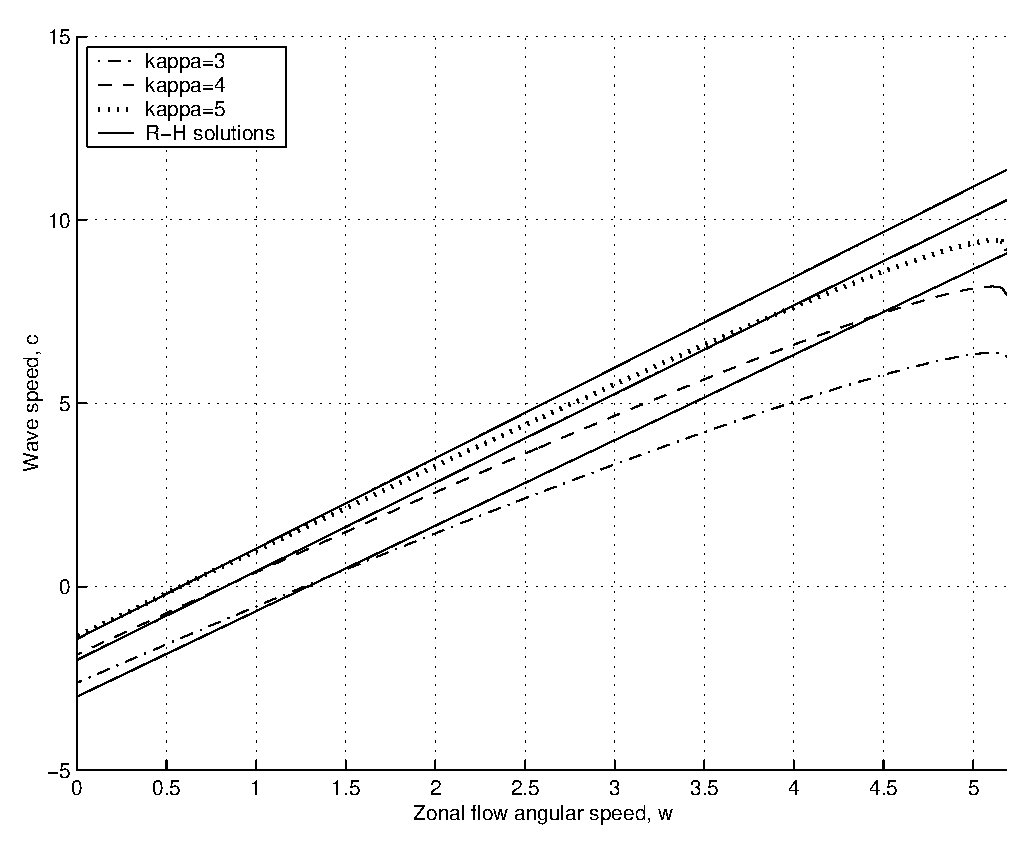
\includegraphics[scale=0.49]{wvchconst1.eps}
\end{figure}
\end{slide}

\tsectionandpart{Nonlinear Theory}

\begin{slide}{Series Solution}
Seek solutions of the full nonlinear problem using Fourier series of the form
\begin{align*}
u_{\lambda}(\eta,\phi) &= \omega\cos\phi+\sum_{m=1}^M \sum_{n=1}^N P_{m,n}\cos(\kappa m \eta) \cos\bigl((2n-1)\phi\bigr),\\
u_{\phi}(\eta,\phi) &= \sum_{m=1}^M \sum_{n=1}^N Q_{m,n}\sin(\kappa m \eta) \sin(2n\phi)\\
h(\eta,\phi) &= \sum_{n=0}^N H_{0,n}\cos(2 n \phi) \notag, \\
&\quad+\sum_{m=1}^{M-1} \sum_{n=1}^N H_{m,n} \cos(\kappa m \eta) (-1)^n \left[ \cos(2n\phi)+\cos\bigl(2(n-1)\phi\bigr) \right].
\end{align*}
\end{slide}

\begin{slide}{Amplitude Forcing and Measurement}
\begin{itemize}
\item Force amplitude $\mathcal{A}$ through either $H_{1,1}$ or $c$.
\item In this context, progressive Rossby waves are perturbations from a base Westerly zonal flow, for which the height contours are simply circles of constant $\phi$. The unperturbed free-surface height contours at $\phi=\pm\pi/4$ are taken here as the base level, against which Rossby wave amplitudes are measured.
\item Define the equatorial, polar and average amplitudes as $\mathcal{A}_{e}$, $\mathcal{A}_{p}$ and $\mathcal{A}_{ave}$ respectively.
\end{itemize}
\end{slide}

\begin{slide}{Solution Process}
\begin{itemize}
\item Solve using Collocation. We evaluate the three governing dynamical equations at every point of the collocation mesh to give a vector of residuals. In addition, the volume specification equation is evaluated and appended to this vector.
\item Residual equations are solved using a multi-dimensional Newton method.
\item Linearized solutions are used to initialise the Newton method when the amplitude is small.
\item Once a nonlinear solution has been found, the amplitude is slowly increased and bootstrapping is used to trace out the wavespeed versus amplitude curve incrementally.
\end{itemize}
\end{slide}

\begin{slide}{Results for $\kappa=4$, $\omega=1.25$}

\begin{figure}
\psfrag{Ap}{\tiny $\mathcal{A}_{p}$}
\psfrag{Ae}{\tiny $\mathcal{A}_{e}$}
\psfrag{Aave}{\tiny $\mathcal{A}_{ave}$}
\psfrag{Wavespeed}{\scriptsize Wavespeed, $c$}
\psfrag{Amplitude}{\scriptsize Amplitude (deg.)}
\psfrag{Linearised}{\tiny Linearized solution}
	\centering
		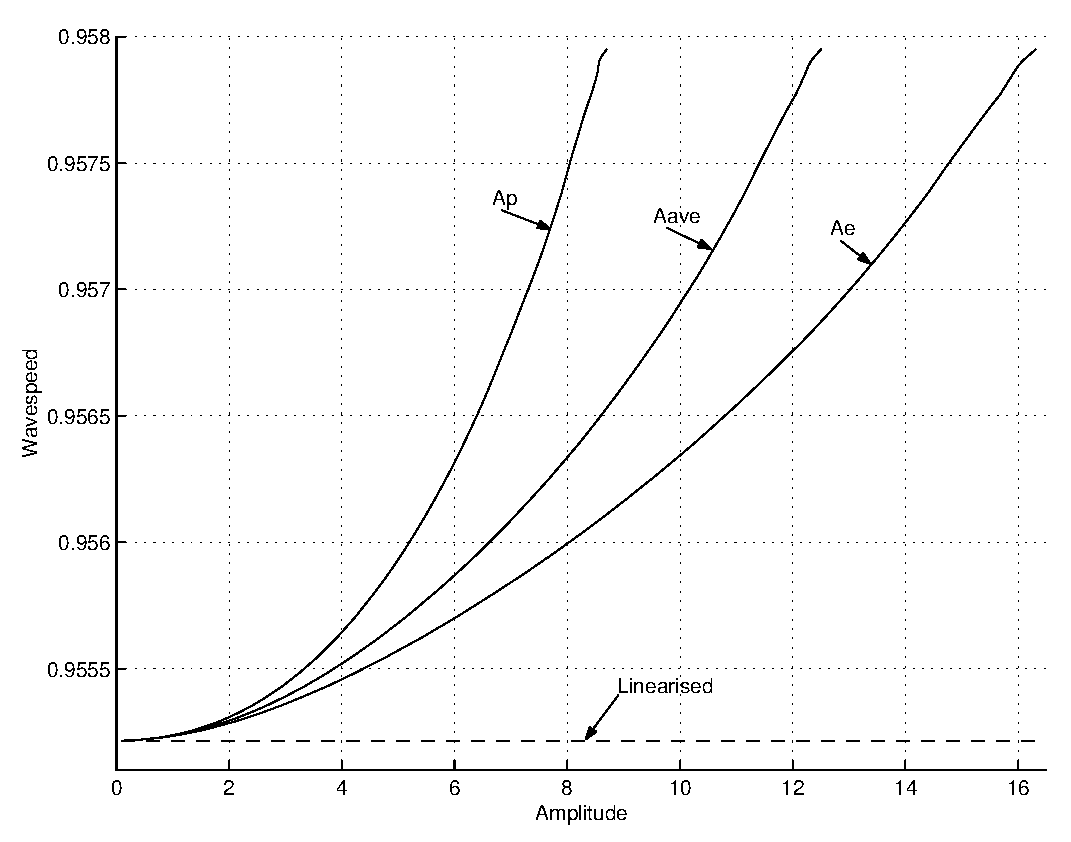
\includegraphics[scale=0.49]{CvsAk4w125.eps}
	\end{figure}

\end{slide}

\begin{slide}{F-S contours, $\kappa=4$, $\omega=1.25$}
\begin{figure}
	\centering
		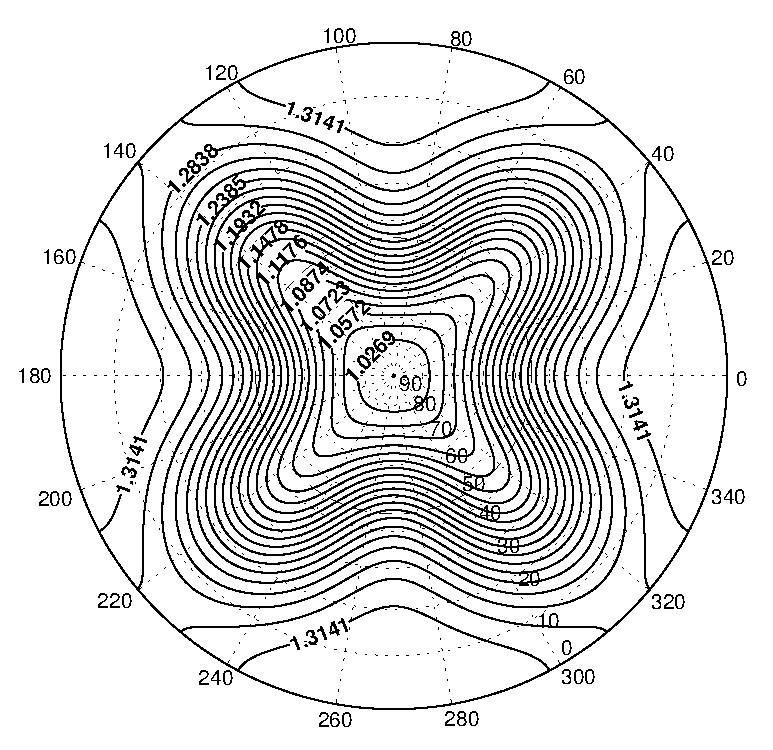
\includegraphics[scale=0.55]{k4w125fsend.eps}
	\end{figure}
\end{slide}

\begin{slide}{Results for $\kappa=4$, $\omega=1.0$}

\begin{figure}
\psfrag{Ap}{\tiny $\mathcal{A}_{p}$}
\psfrag{Ae}{\tiny $\mathcal{A}_{e}$}
\psfrag{Aave}{\tiny $\mathcal{A}_{ave}$}
\psfrag{Wavespeed}{\scriptsize Wavespeed, $c$}
\psfrag{Amplitude}{\scriptsize Amplitude (deg.)}
\psfrag{Linearised}{\tiny Linearized solution}
\psfrag{B1}{\tiny Branch 1}
\psfrag{B2}{\tiny Branch 2}
\psfrag{B3}{\tiny Branch 3}
\psfrag{B4}{\tiny Branch 4}
\psfrag{B5}{\tiny Branch 5}
	\centering
		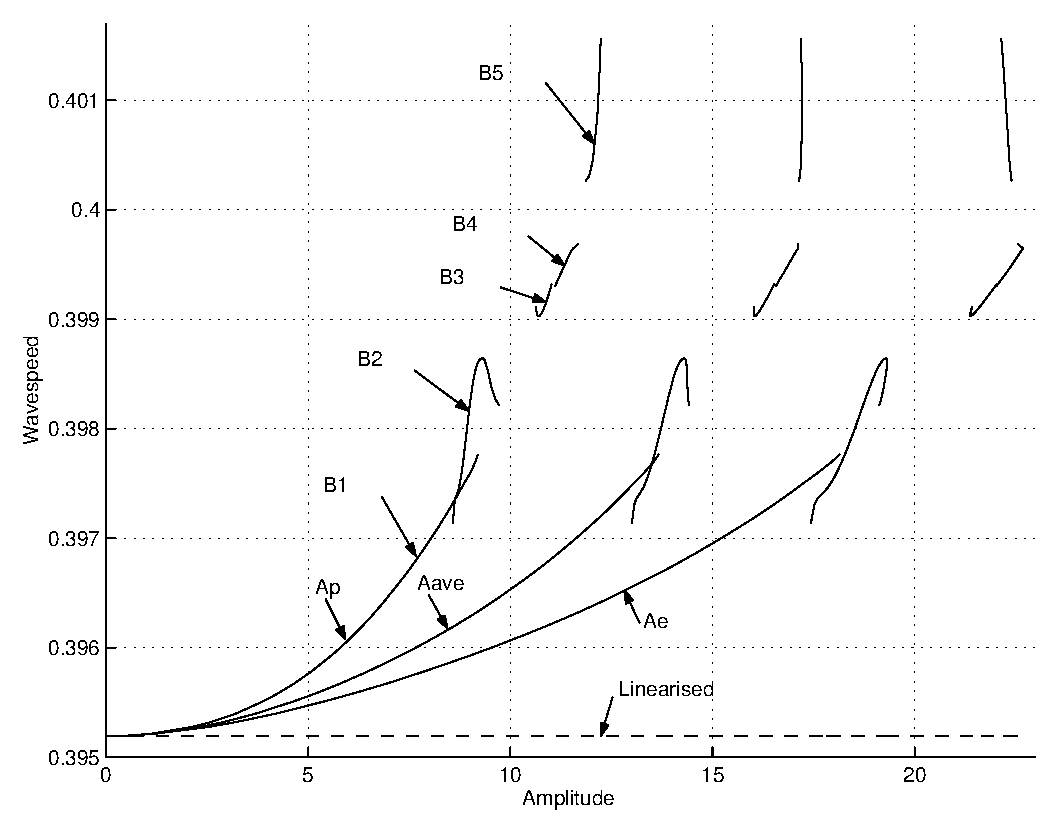
\includegraphics[scale=0.49]{CvsAk4w1.eps}
\end{figure}
\end{slide}

\begin{slide}{F-S contours (end Branch 4), $\kappa=4$, $\omega=1.0$}
\begin{figure}
	\centering
		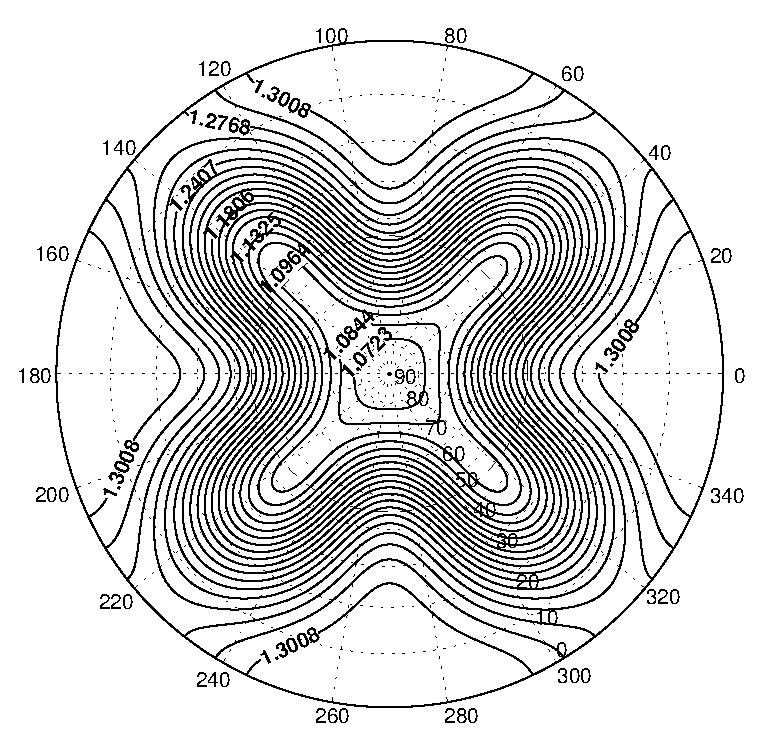
\includegraphics[scale=0.55]{k4w1fsb4end.eps}
	\end{figure}
\end{slide}

\begin{slide}{F-S contours (end Branch 5), $\kappa=4$, $\omega=1.0$}
\begin{figure}
	\centering
		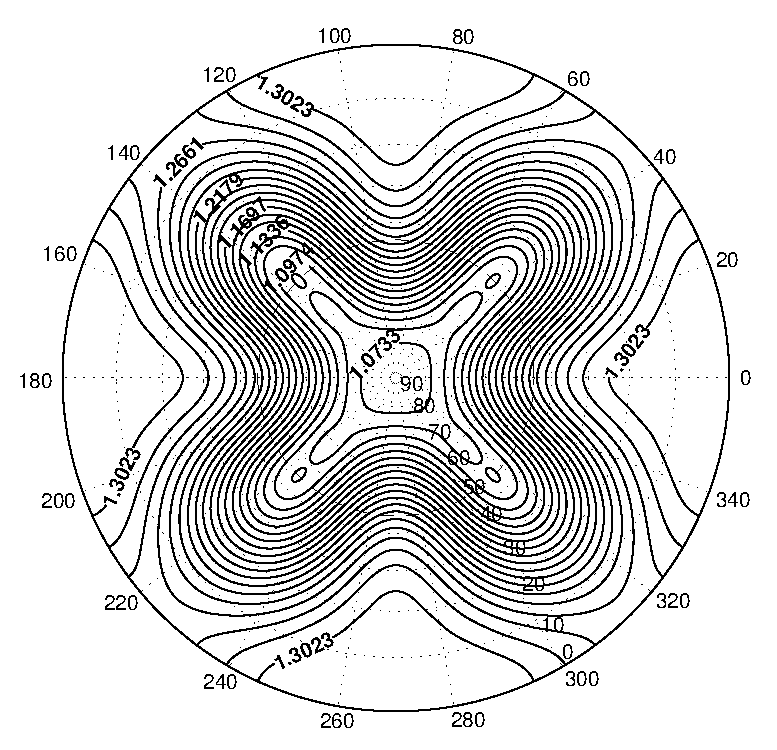
\includegraphics[scale=0.55]{k4w1fsb5end.eps}
	\end{figure}
\end{slide}


\begin{slide}{Velocity (end Branch 5), $\kappa=4$, $\omega=1.0$}
\begin{figure}
\psfrag{Stagnation points}{\scriptsize Stagnation points}
\psfrag{Reverse Flow}{\scriptsize Reverse flow}
	\centering
		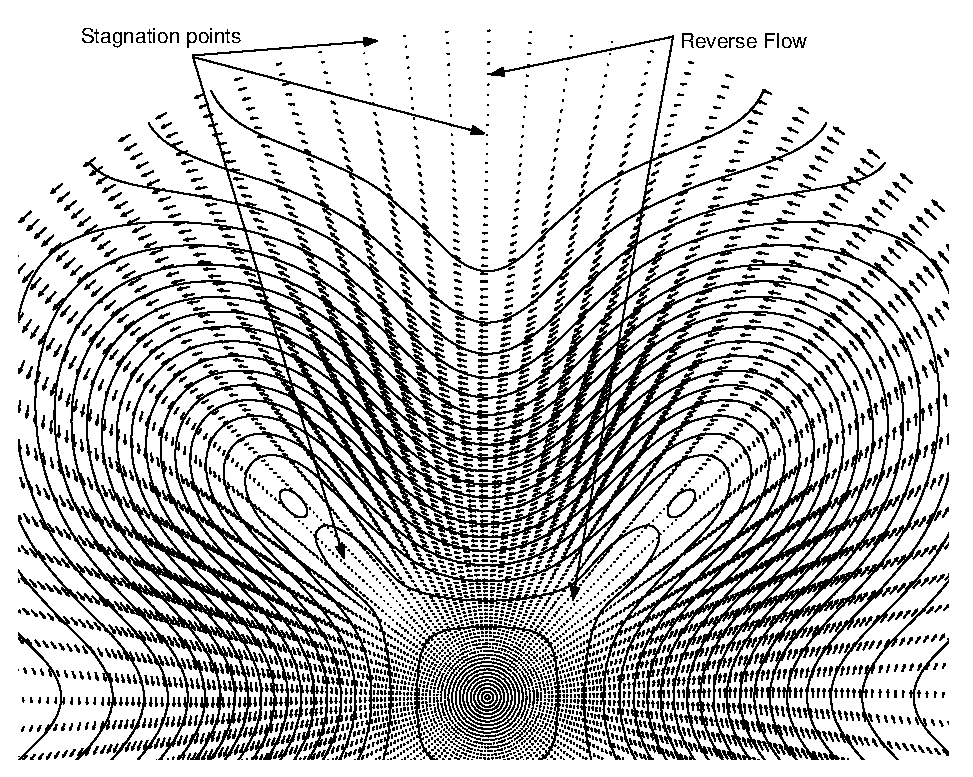
\includegraphics[scale=0.54]{k4w1fsvvb5end.eps}
\end{figure}
\end{slide}

\end{document}
